\section{Résultats}
\label{sec:results}
% =====================================================================

\subsection{Mocks de type DESI : ASTRA split, density split et 2PCF}

Le Tableau~\ref{tab:sigma} et la Figure~\ref{fig:ratios} donnent les prévisions de référence. Les deux méthodes améliorent la 2PCF de facteurs 1.6--3.1 selon le paramètre. Entre elles, le rapport $\sigma_{\rm DS}/\sigma_{\rm ASTRA}$ pour les corrélations croisées des quartiles aléatoires vaut 0.90, 1.10, 0.84, 0.83, 0.94 et 0.92 pour $\omega_b$, $\omega_{\rm cdm}$, $n_s$, $\sigma_8$, $w_0$ et $w_a$ : le density split est légèrement en avance, de 5--15\%, sauf sur $\omega_{\rm cdm}$. Les deux sont clairement complémentaires : combinées, elles améliorent la meilleure des deux de 23\% ($\sigma_8$) à un facteur 2.4 ($\omega_b$), 1.4 et 1.7 pour $w_0$ et $w_a$, et la combinaison avec la 2PCF est la plus contraignante (Figure~\ref{fig:combined}). Les erreurs sur $w_0$ et $w_a$ ($\simeq0.8$ et $2.7$ pour un volume de $(500\Mpch)^3$) sont plus grandes que l'étendue de la suite AbacusSummit : à ce volume, les paramètres d'énergie noire ne sont pas contraints, et seul le contenu relatif en information des statistiques a un sens. Les ajouter garde néanmoins modérées les erreurs d'ASTRA sur les autres paramètres (au plus $+40\%$, sur $\omega_{\rm cdm}$) et laisse stables les rapports DS/ASTRA, de sorte que la comparaison ne dépend pas de la liberté de $w_0$ et $w_a$. Les variantes (auto-corrélations, quartiles de galaxies, environnements isolés) donnent des rapports compris entre 0.5 et 1.4 sans gagnant constant (Figure~\ref{fig:ratios}).

\begin{table}[!htbp]
\centering\small
\begin{tabular}{lcccccc}
\toprule
vecteur de données & $\omega_b$ & $\omega_{\rm cdm}$ & $n_s$ & $\sigma_8$ & $w_0$ & $w_a$ \\
\midrule
2PCF & 0.033 & 0.057 & 0.40 & 0.58 & 2.1 & 6.7 \\
ASTRA & 0.012 & 0.032 & 0.22 & 0.23 & 0.80 & 2.7 \\
DS & 0.011 & 0.035 & 0.18 & 0.19 & 0.75 & 2.5 \\
ASTRA + DS & 0.0046 & 0.022 & 0.13 & 0.15 & 0.53 & 1.5 \\
2PCF + ASTRA + DS & 0.0039 & 0.019 & 0.12 & 0.13 & 0.50 & 1.3 \\
\bottomrule
\end{tabular}
\caption{Erreurs marginalisées à $1\sigma$ de référence (corrélations croisées Q1+Q4 des quartiles aléatoires, HOD marginalisée) pour un volume de $(500\Mpch)^3$. Ces valeurs sont comparables aux largeurs des priors et comparent le contenu en information ; ce ne sont pas des contraintes réalistes.}
\label{tab:sigma}
\end{table}

La Figure~\ref{fig:triangle} montre les contours correspondants : les statistiques d'environnement réduisent principalement les dégénérescences $\omega_b$--$\omega_{\rm cdm}$ et $n_s$--$\sigma_8$ de la 2PCF.

\paragraph{Quartiles individuels.} Les Figures~\ref{fig:q_astra} et~\ref{fig:q_ds} montrent, comme dans les analyses de density split, les contraintes de chaque quartile seul et des quatre ensemble, et les Figures~\ref{fig:c_astra} et~\ref{fig:c_ds} comparent la 2PCF, les quartiles de type vide (Q1) et de type amas (Q4), tous les quartiles, et tous les quartiles avec la 2PCF. Un quartile seul contraint les paramètres à peu près aussi bien que la 2PCF, les quartiles intermédiaires (Q3 en particulier) étant les moins contraignants, mais son information est de nature différente : la 2PCF moyenne le clustering sur tous les environnements, alors qu'un quartile le mesure autour d'un seul intervalle de densités, par exemple le profil des galaxies autour des vides pour Q1. Chaque environnement répond aux paramètres à sa manière : les quartiles de vides et d'amas répondent avec des signes opposés et des dépendances en échelle différentes (Figures~\ref{fig:der_astra}, \ref{fig:der_ds}), et leurs directions de dégénérescence diffèrent. Le gain provient donc de la combinaison des environnements : les quatre quartiles ensemble sont plusieurs fois plus serrés que chacun d'eux ou que la 2PCF, qui mélange tous les environnements et perd cette distinction. La Figure~\ref{fig:quartiles} résume l'information par environnement : les corrélations croisées Q4 seules battent déjà la 2PCF sur la plupart des paramètres, Q1 et Q4 ensemble doublent le gain, et l'ajout des auto-corrélations le multiplie encore.

\paragraph{Auto-corrélations.} L'ajout des auto-corrélations des quartiles aux corrélations croisées resserre les contraintes des deux méthodes de facteurs 1.3--2.8 selon le paramètre (Figure~\ref{fig:autocross}) ; avec elles, les deux méthodes restent comparables (rapports 0.7--1.1), le density split étant en avance sur $\omega_b$, $\omega_{\rm cdm}$ et $n_s$ et ASTRA sur $\sigma_8$.

\paragraph{Coupures en échelle.} La Figure~\ref{fig:smin} montre les erreurs en fonction de l'échelle minimale. Toutes les statistiques perdent de l'information lorsque les petites échelles sont retirées, les statistiques d'environnement restant 0.2--0.5 dex sous la 2PCF jusqu'à $s_{\min}=70\Mpch$ (au-delà, la 2PCF a moins de bins que de paramètres). ASTRA et density split restent à moins de 0.1 dex l'un de l'autre pour toutes les coupures, leur classement changeant avec $s_{\min}$, et leur combinaison conserve son avantage de 0.2--0.4 dex.

\paragraph{Point fiduciel.} Évalué à quatre HOD différentes, le rapport $\sigma_{\rm DS}/\sigma_{\rm ASTRA}$ reste entre 0.77 et 1.14 pour les six paramètres (Tableau~\ref{tab:covbox} ; 0.75--1.11 avec quatre paramètres) : le point fiduciel compte au niveau de $\pm15\%$.

\begin{table}[!htbp]
\centering\small
\begin{tabular}{lcccccc}
\toprule
HOD fiducielle & $\omega_b$ & $\omega_{\rm cdm}$ & $n_s$ & $\sigma_8$ & $w_0$ & $w_a$ \\
\midrule
officielle & 0.90(11) & 1.10(16) & 0.84(15) & 0.83(10) & 0.94(11) & 0.92(9) \\
\texttt{hod239} & 0.83(9) & 0.92(7) & 1.04(12) & 0.93(8) & 0.88(6) & 0.84(8) \\
\texttt{hod212} & 0.77(7) & 0.94(9) & 0.94(13) & 0.84(8) & 0.85(8) & 0.89(10) \\
\texttt{hod795} & 0.79(8) & 0.98(10) & 1.06(16) & 1.14(10) & 0.89(12) & 0.92(13) \\
\bottomrule
\end{tabular}
\caption{$\sigma_{\rm DS}/\sigma_{\rm ASTRA}$ (au-dessus de 1 : ASTRA en avance) pour les corrélations croisées des quartiles aléatoires avec la covariance officielle à quatre HOD fiducielles ; entre parenthèses, l'incertitude due à l'entraînement de l'émulateur.}
\label{tab:covbox}
\end{table}

\begin{figure}[!htbp]
\centering
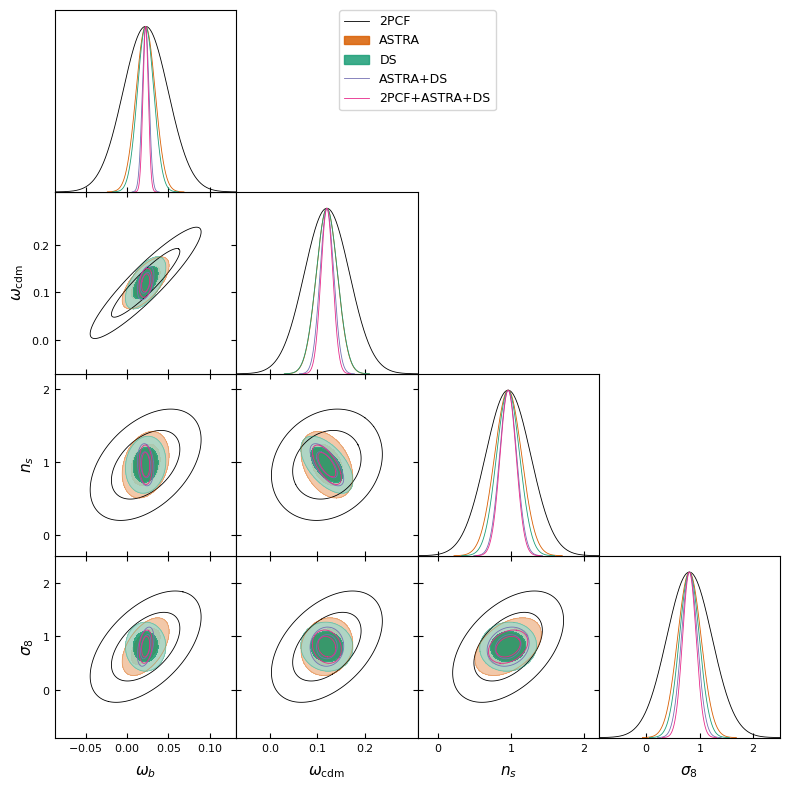
\includegraphics[width=\linewidth]{v2_triangle.png}
\caption{Contours de Fisher de référence (68\% et 95\%) pour la 2PCF, l'ASTRA split, le density split et leurs combinaisons, un volume de $(500\Mpch)^3$, HOD marginalisée.}
\label{fig:triangle}
\end{figure}

\begin{figure}[!htbp]
\centering
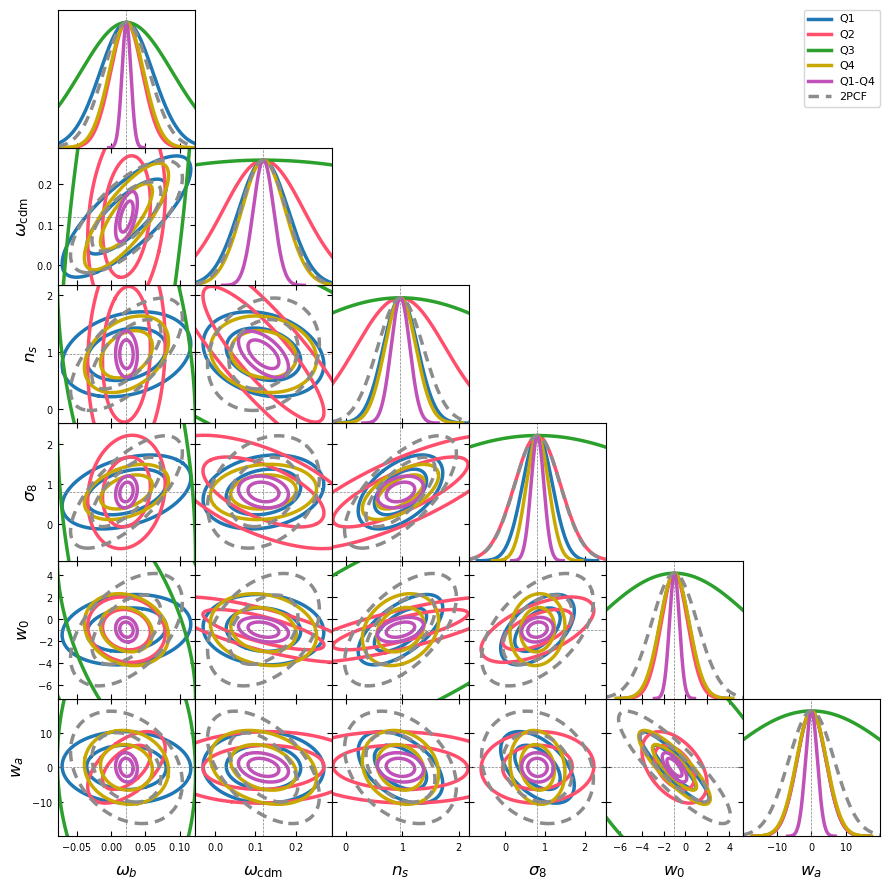
\includegraphics[width=\linewidth]{v1style_quartiles_astra.png}
\caption{Contraintes (68\% et 95\%) des quartiles individuels et combinés de l'ASTRA split (corrélations croisées) et de la 2PCF (tirets), référence, HOD marginalisée. Les axes couvrent $\pm3\sigma$ de la 2PCF.}
\label{fig:q_astra}
\end{figure}

\begin{figure}[!htbp]
\centering
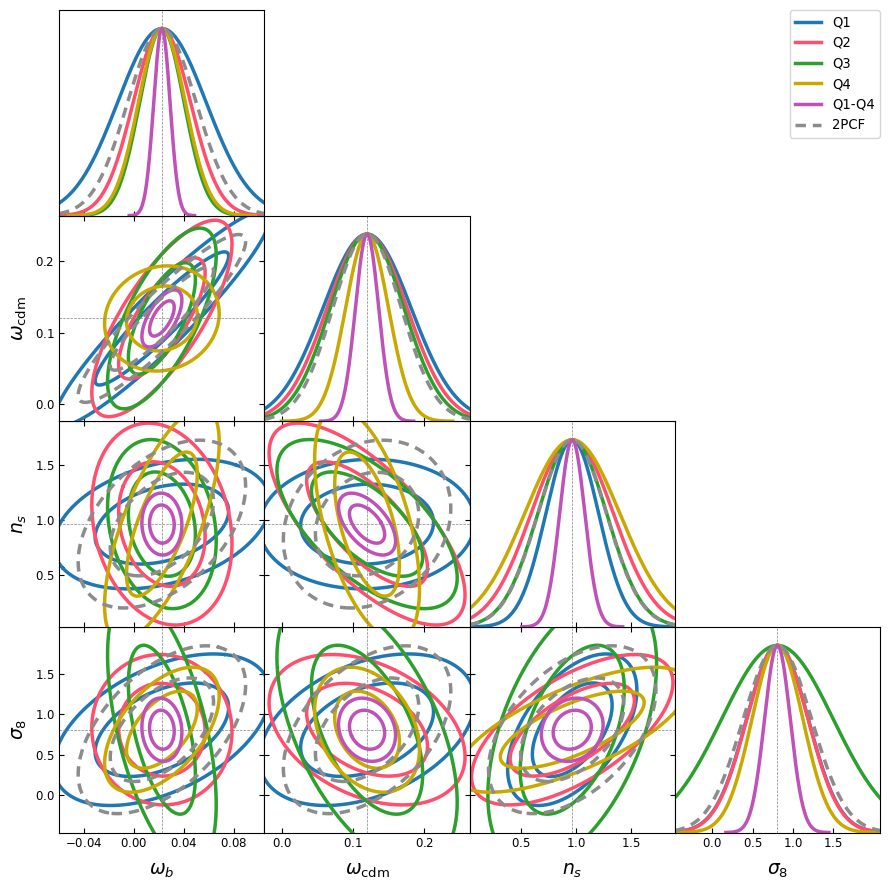
\includegraphics[width=\linewidth]{v1style_quartiles_ds.png}
\caption{Identique à la Figure~\ref{fig:q_astra} pour le density split.}
\label{fig:q_ds}
\end{figure}

\begin{figure}[!htbp]
\centering
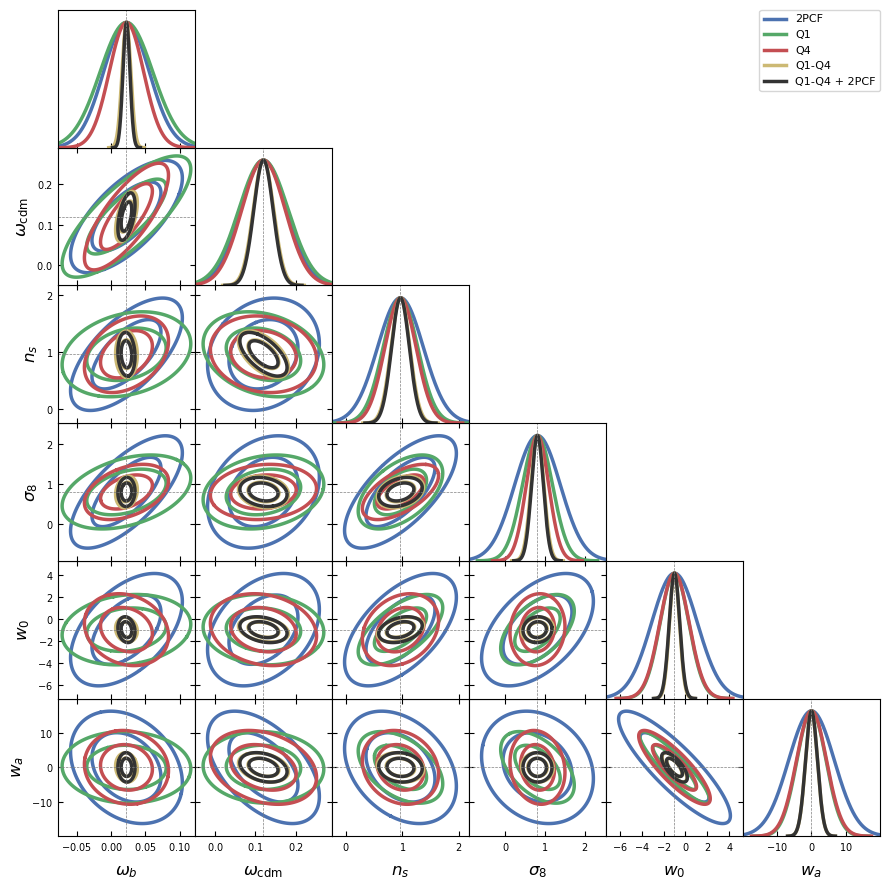
\includegraphics[width=\linewidth]{v1style_constraints_astra.png}
\caption{ASTRA split : contraintes de la 2PCF, des corrélations croisées Q1 et Q4, de tous les quartiles, et de tous les quartiles avec la 2PCF (référence).}
\label{fig:c_astra}
\end{figure}

\begin{figure}[!htbp]
\centering
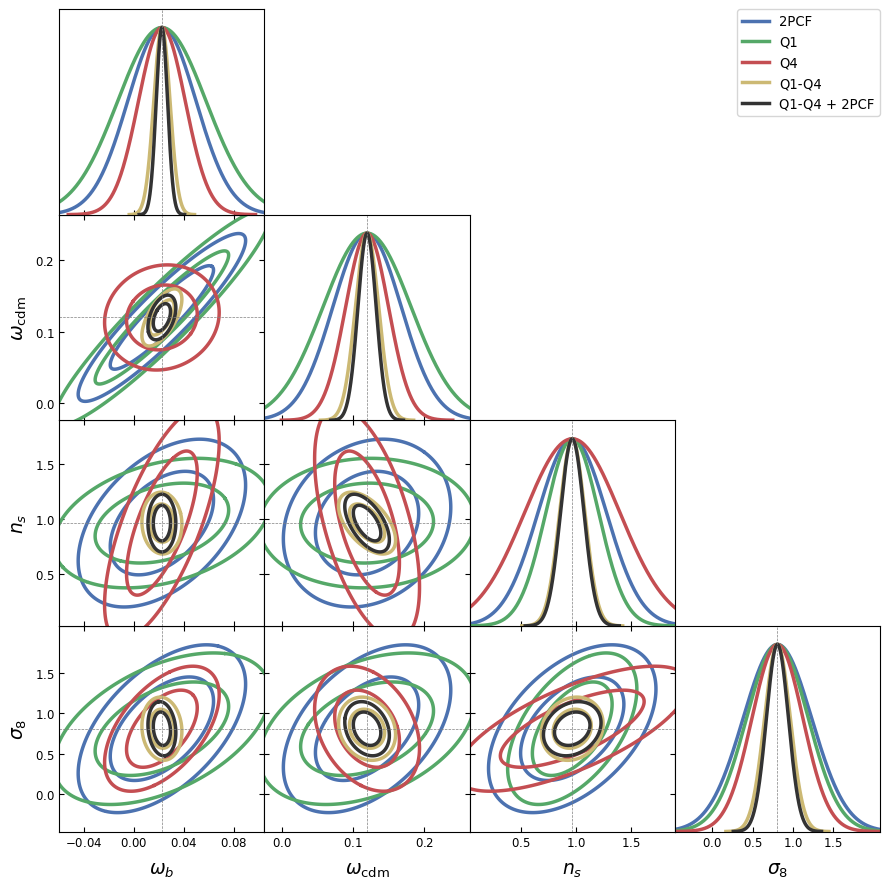
\includegraphics[width=\linewidth]{v1style_constraints_ds.png}
\caption{Identique à la Figure~\ref{fig:c_astra} pour le density split.}
\label{fig:c_ds}
\end{figure}

\begin{figure*}[!tp]
\centering
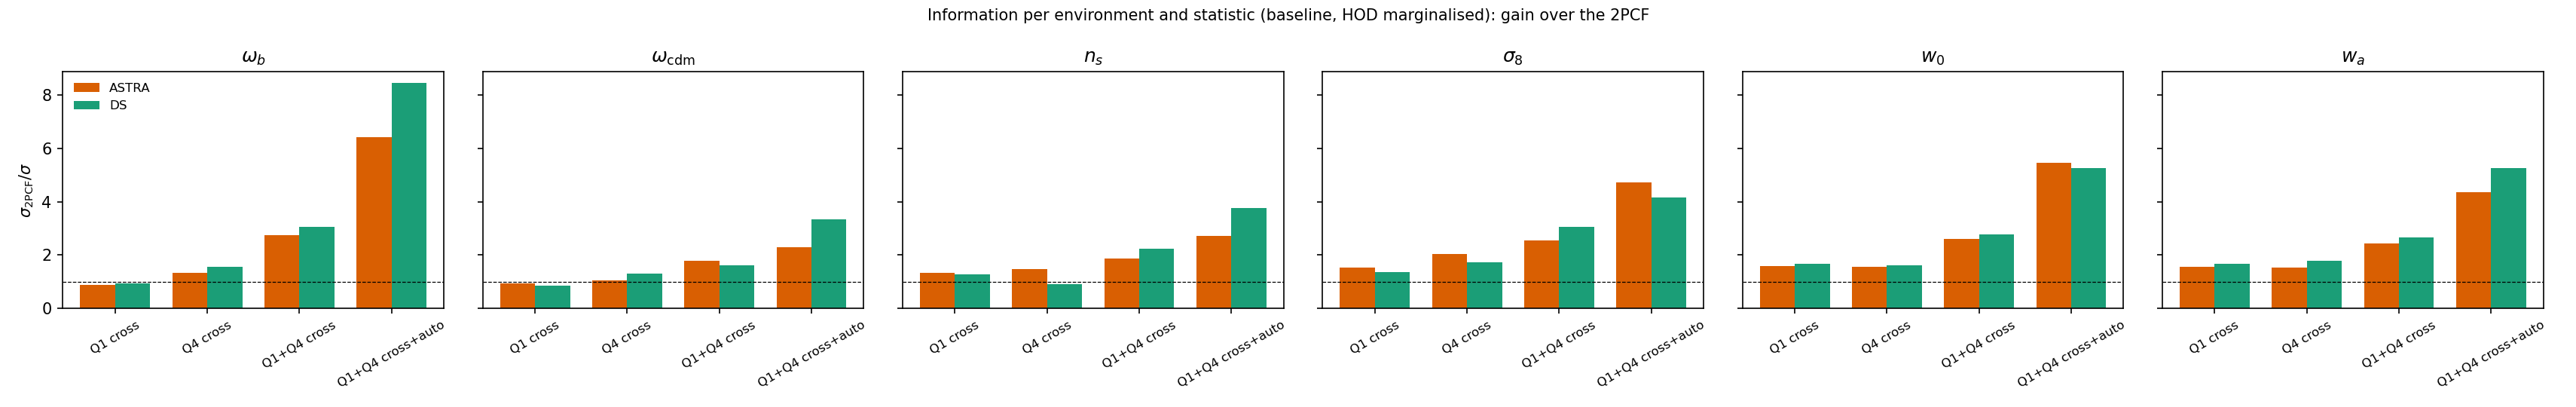
\includegraphics[width=\textwidth]{v2_quartiles.png}
\caption{Gain par rapport à la 2PCF, $\sigma_{\rm 2PCF}/\sigma$, pour les corrélations croisées Q1 et Q4 seules, ensemble, et avec les auto-corrélations des quartiles, pour l'ASTRA split (orange) et le density split (vert) (référence, HOD marginalisée).}
\label{fig:quartiles}
\end{figure*}

\begin{figure}[!htbp]
\centering
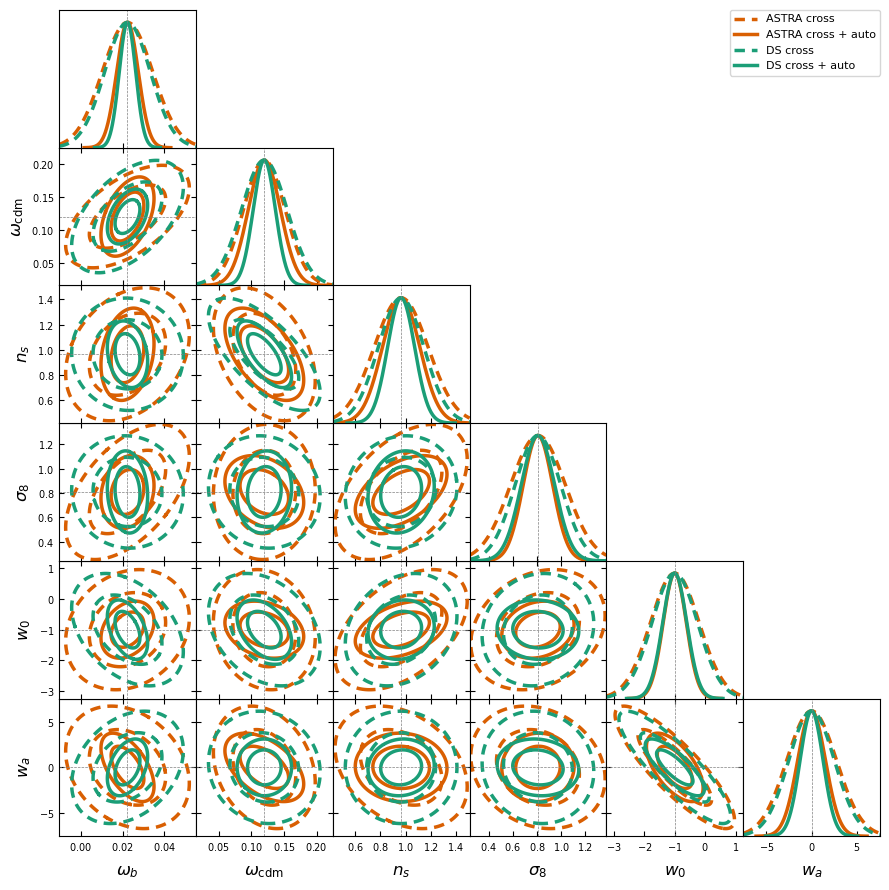
\includegraphics[width=\linewidth]{v1style_autocross.png}
\caption{Corrélations croisées Q1+Q4 seules (tirets) et avec les auto-corrélations des quartiles (trait plein), pour l'ASTRA split (orange) et le density split (vert), référence.}
\label{fig:autocross}
\end{figure}

\begin{figure}[!htbp]
\centering
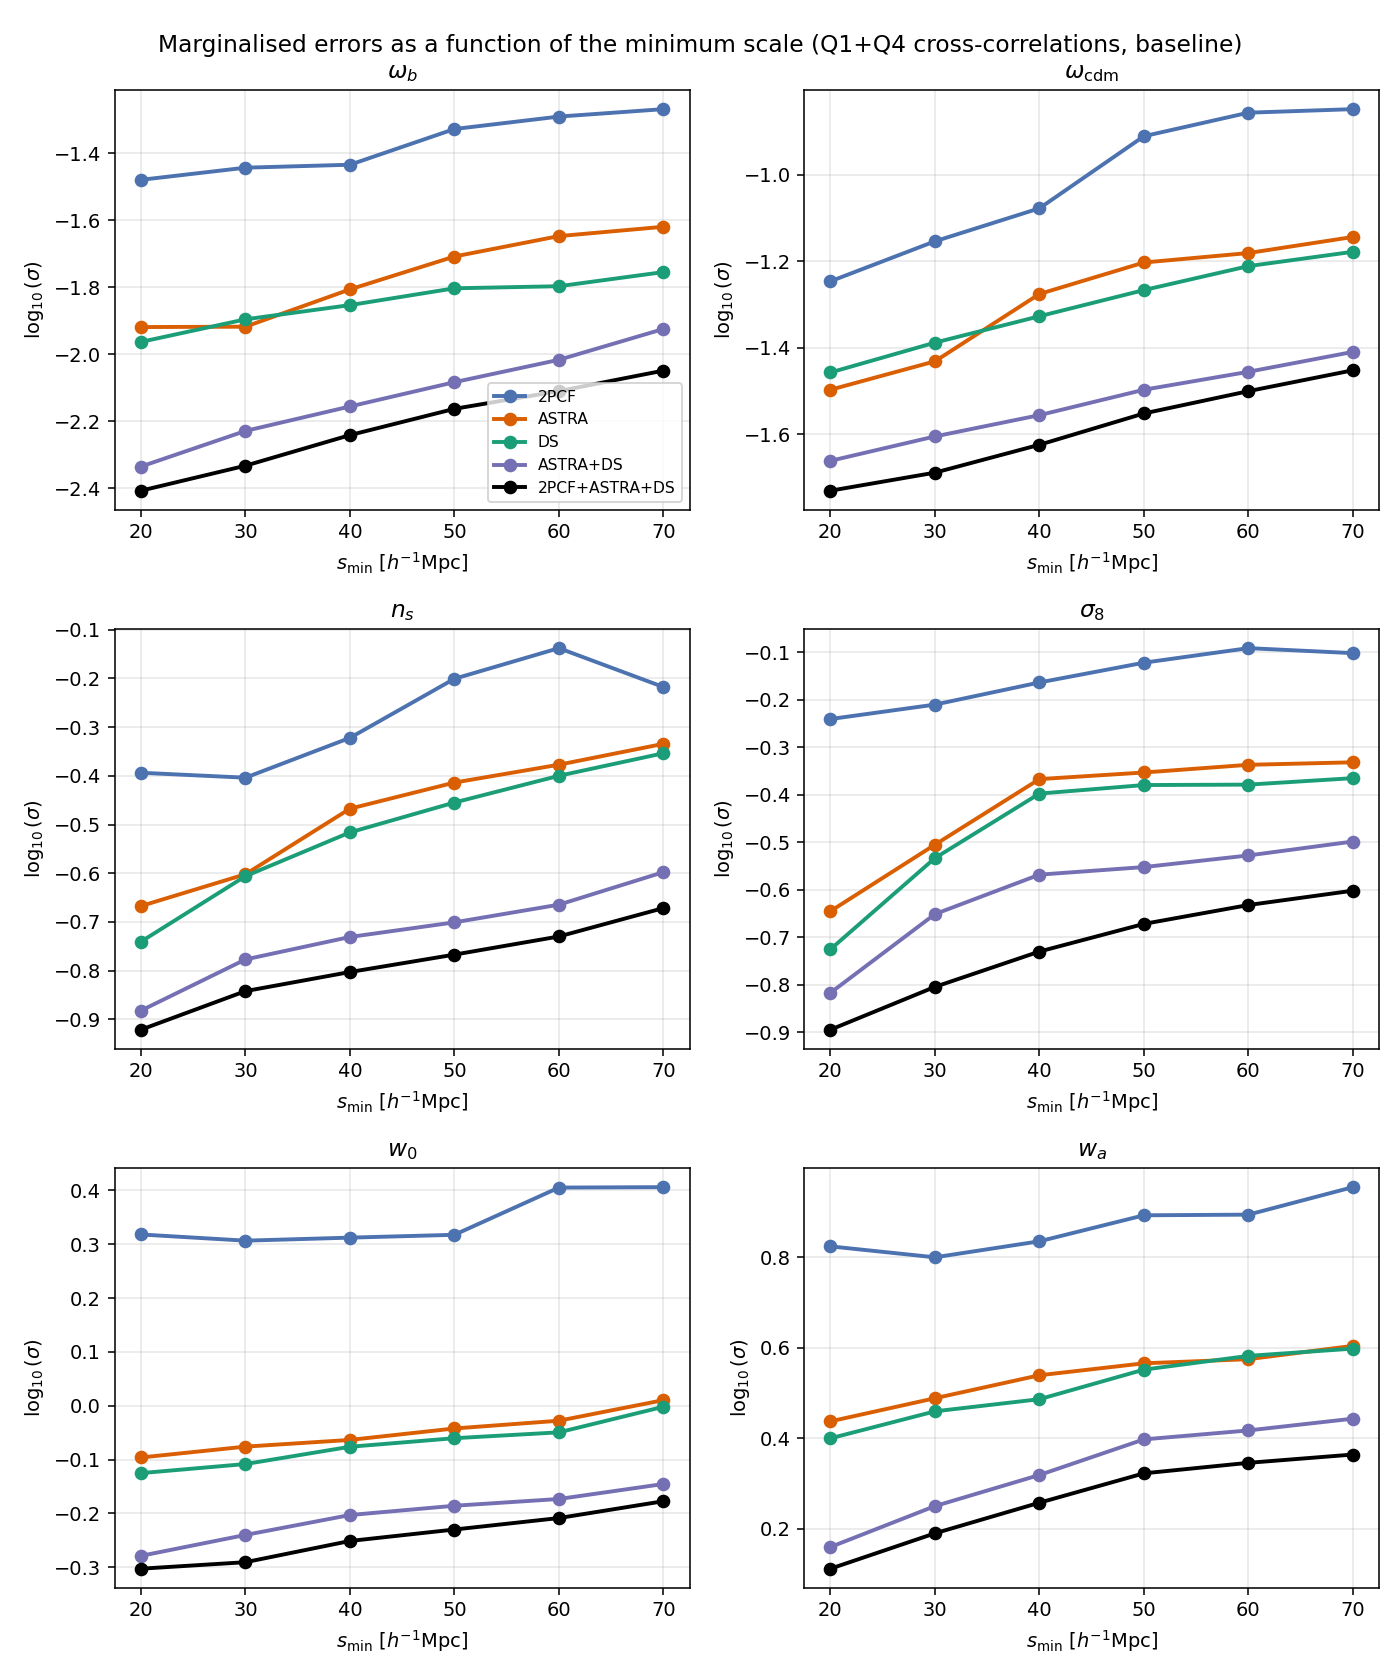
\includegraphics[width=\linewidth]{v1style_smin.png}
\caption{Erreurs marginalisées en fonction de l'échelle minimale $s_{\min}$ (corrélations croisées Q1+Q4, référence).}
\label{fig:smin}
\end{figure}

\begin{figure*}[!tp]
\centering
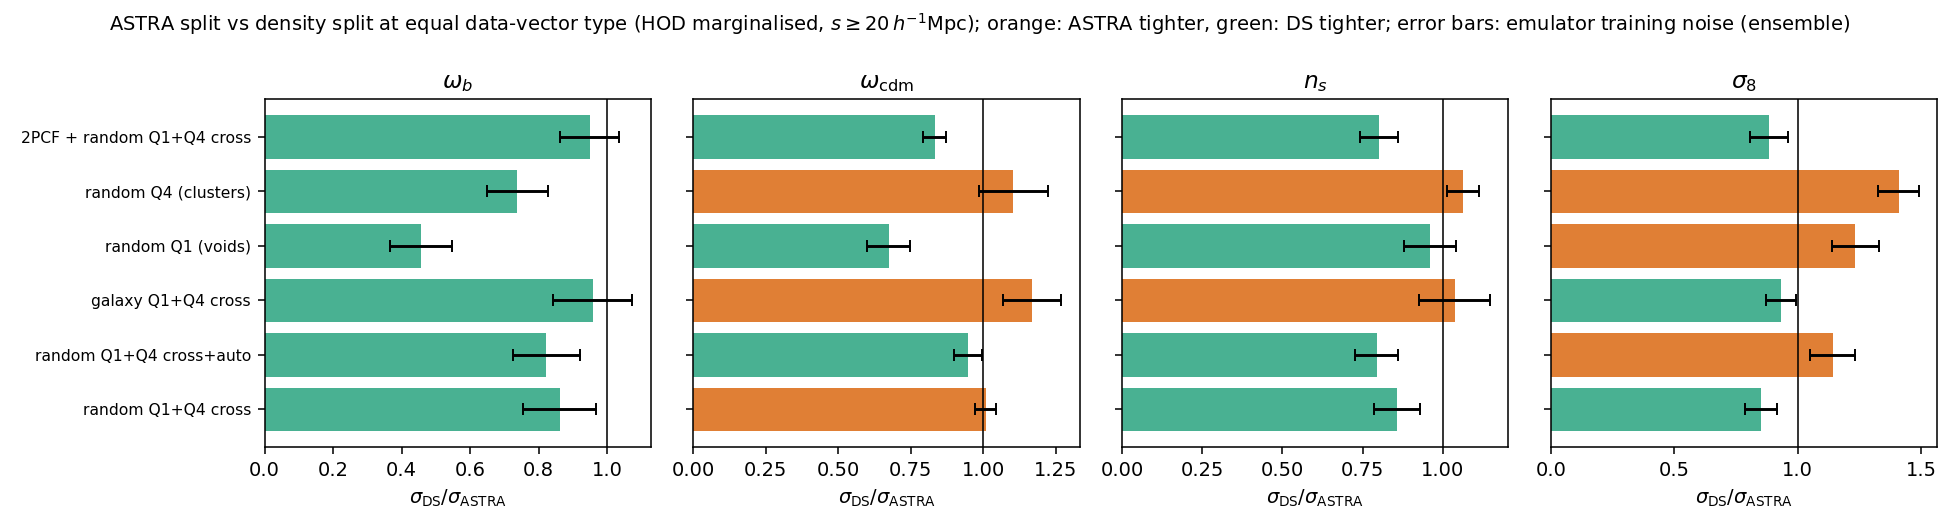
\includegraphics[width=\textwidth]{v2_compare_ratios.png}
\caption{Référence : $\sigma_{\rm DS}/\sigma_{\rm ASTRA}$ pour plusieurs types de vecteurs de données (au-dessus de 1 : l'ASTRA split est plus contraignant). Barres d'erreur : incertitude due à l'entraînement de l'émulateur.}
\label{fig:ratios}
\end{figure*}

\begin{figure*}[!tp]
\centering
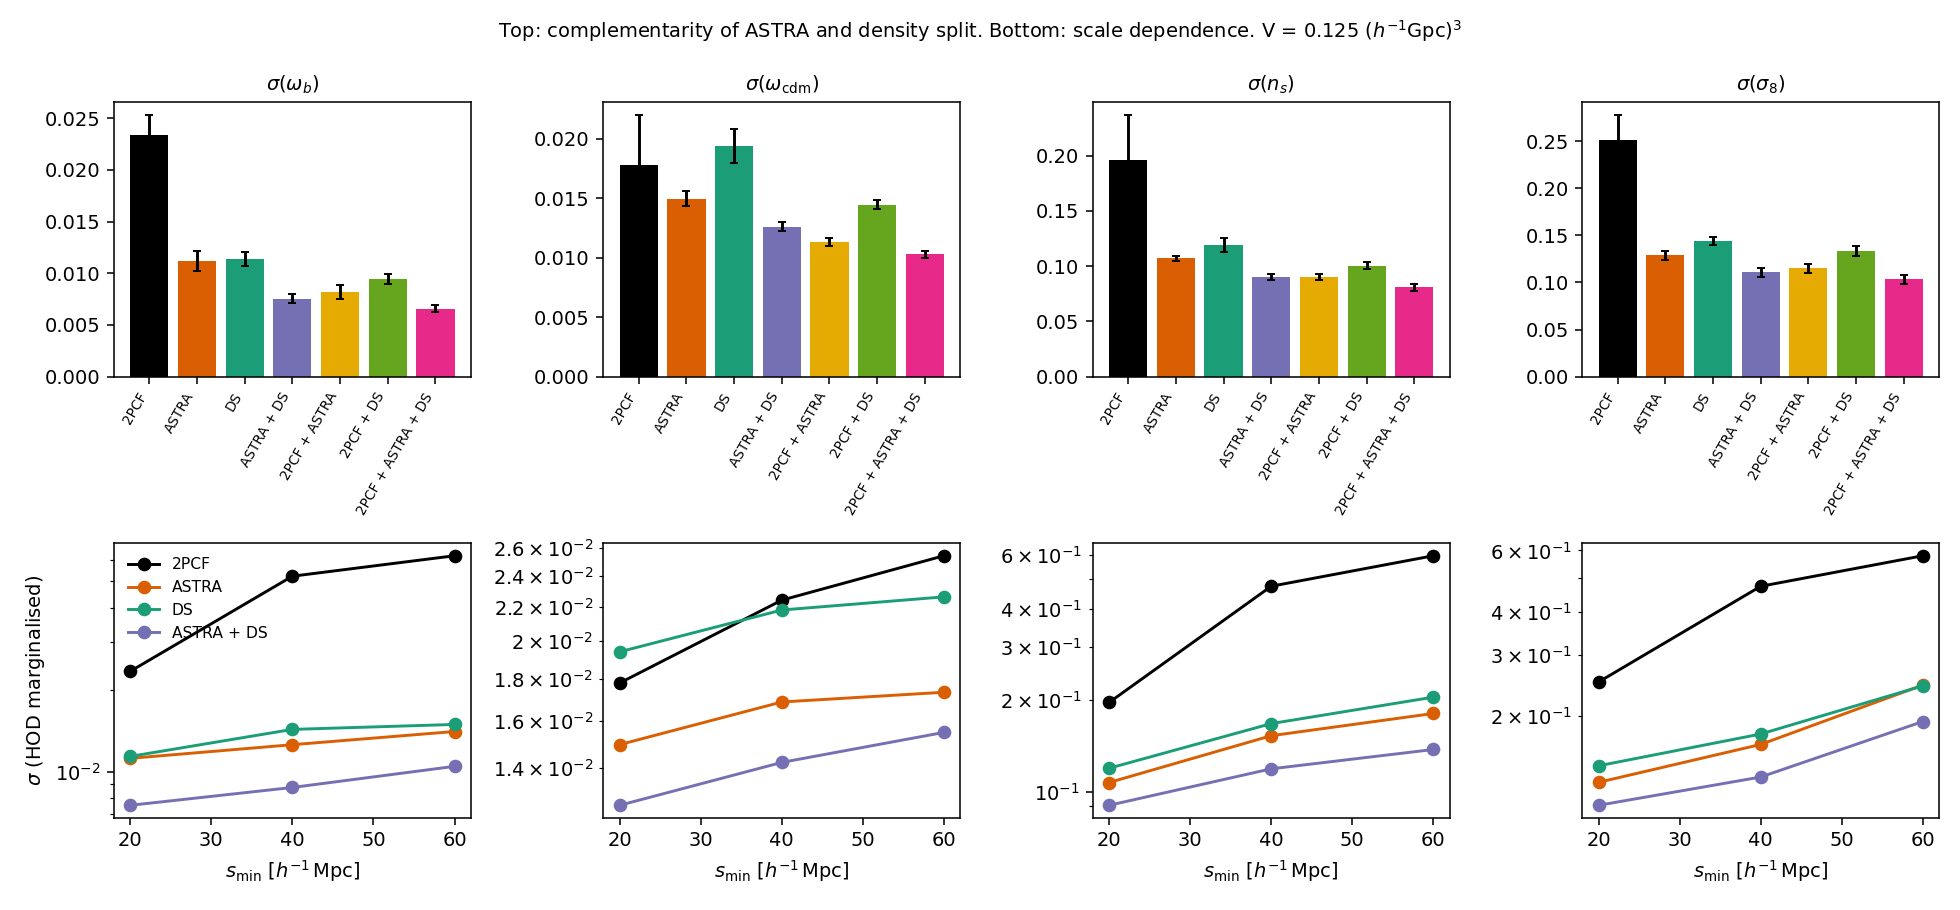
\includegraphics[width=\textwidth]{v2_compare_combined.png}
\caption{Référence. Haut : erreurs marginalisées de la 2PCF, de l'ASTRA split, du density split et de leurs combinaisons. Bas : dépendance en l'échelle minimale.}
\label{fig:combined}
\end{figure*}

\subsection{Halos de Quijote}
\label{sec:quijote}

\paragraph{Covariance.} Avec 4000 réalisations fiducielles, la covariance est convergée : à dérivées fixées, les erreurs marginalisées changent de moins de 1\% entre 2000 et 4000 réalisations, et de moins de 6\% entre 1000 et 4000. (Environ la moitié des 15\,517 catalogues fiduciels de notre copie étaient vides, un téléchargement incomplet sans conséquence vu cette convergence ; tous les ensembles de dérivées sont complets.)

\paragraph{Appariement.} Les réalisations $\pm$ d'un indice donné partagent leurs conditions initiales : la dispersion des différences entre réalisations de même indice est 3 à 4 fois plus petite qu'entre indices différents, pour la 2PCF comme pour les statistiques de quartiles.

\paragraph{Bruit des dérivées.} Même appariées, les dérivées restent bruitées. Quijote est conçu pour des statistiques des champs de matière et de halos (spectre de puissance, bispectre, \dots). Nos observables ajoutent deux sources de bruit que l'appariement ne peut annuler :
\begin{enumerate}
\item \emph{Traceurs épars.} Avec $\simeq50\,000$ halos hôtes par $(h^{-1}{\rm Gpc})^3$, chaque quartile ne contient que $\simeq12\,000$ halos (ou points aléatoires), et le bruit de Poisson des statistiques de quartiles est grand.
\item \emph{Classification discrète.} Un petit changement de cosmologie déplace des halos et des points aléatoires d'un quartile à l'autre. Cette reclassification n'est que partiellement commune aux simulations $+$ et $-$, même avec des conditions initiales identiques, et ajoute un bruit qui ne s'annule pas dans la différence.
\end{enumerate}
Ce bruit est surtout amplifié par la matrice de Fisher à six paramètres. $\Omega_b$, $h$ et $n_s$ (et $M_\nu$) sont fortement dégénérés dans le clustering des halos : leur combinaison la plus faible est contrainte par une très faible quantité d'information, du même ordre que le bruit restant dans la moyenne de 500 paires de dérivées, de sorte que selon cette direction les dérivées sont dominées par le bruit. L'estimateur de Fisher standard est alors biaisé vers le haut, et la soustraction du terme de bruit attendu rend les matrices à six paramètres non définies positives (Annexe~\ref{app:maths}).

\paragraph{Estimateur et critère de fiabilité.} Nous utilisons donc l'approche de \cite{CoultonWandelt2023} : l'estimateur standard est biaisé vers le haut par le bruit des dérivées, un estimateur comprimé (la moitié des simulations définit la compression, l'autre moitié mesure son information) est biaisé vers le bas ; les deux encadrent l'information de Fisher vraie, et leur moyenne géométrique est presque non biaisée. Là où ils s'accordent, la prévision ne dépend pas du bruit des dérivées : nous appelons une prévision \emph{fiable} lorsque les erreurs comprimée et standard diffèrent de moins d'un facteur 1.5 pour les deux statistiques comparées.

\paragraph{Choix des paramètres.} Le biais croît avec la longueur du vecteur de données et se concentre dans les directions dégénérées. Nous avons calculé les prévisions pour six sous-ensembles de paramètres, de $(\Omega_m,\sigma_8)$ aux six paramètres, et trois compressions du vecteur de données (bins de $10\Mpch$ avec $\ell=0,2$ ; bins de $20\Mpch$ avec $\ell=0,2$ ; bins de $20\Mpch$, monopôle seul ; Figure~\ref{fig:qsubsets}). Seuls $(\Omega_m,\sigma_8)$ et $(\Omega_m,n_s,\sigma_8)$ donnent des prévisions fiables, pour toutes les compressions ; dès que $\Omega_b$, $h$ ou $M_\nu$ sont variés, les deux estimateurs diffèrent de facteurs 2--10 et le classement des méthodes change d'une compression à l'autre. Ces paramètres ne peuvent pas être contraints avec ces observables et 500 paires de dérivées. Fixer $\Omega_b$, $h$ (et $n_s$), comme le font de nombreuses prévisions de density split, se justifie par des contraintes externes (BBN, CMB) ; $M_\nu$ exigerait des traceurs plus denses ou beaucoup plus de simulations de dérivées.

\paragraph{Résultats.} Les prévisions fiables (Tableau~\ref{tab:quijote}) s'accordent avec l'analyse de type DESI pour les corrélations croisées des quartiles aléatoires : le density split est aussi contraignant que l'ASTRA split ou plus ($\sigma_{\rm DS}/\sigma_{\rm ASTRA}=0.6$--$1.1$). Lorsque les auto-corrélations des quartiles sont ajoutées, ou avec les quartiles de halos, l'ASTRA split est plus contraignant sur $\sigma_8$ d'un facteur 1.5--2 et comparable sur $\Omega_m$ et $n_s$ : son information réside davantage dans le clustering de ses environnements avec eux-mêmes et dans les environnements des traceurs que dans les profils des traceurs autour d'environnements aléatoires.

\begin{table}[!htbp]
\centering\small
\begin{tabular}{llccc}
\toprule
quartiles & paramètres & $\Omega_m$ & $n_s$ & $\sigma_8$ \\
\midrule
aléatoires, croisées & $\Omega_m,\sigma_8$ & 0.86--1.04 & -- & 0.65--0.81 \\
aléatoires, croisées & $\Omega_m,n_s,\sigma_8$ & 0.57--0.64 & 0.68--0.74 & 1.04--1.14 \\
aléatoires, + auto & $\Omega_m,\sigma_8$ & 1.19--1.40 & -- & 1.54--2.11 \\
aléatoires, + auto & $\Omega_m,n_s,\sigma_8$ & 0.74--0.81 & 0.85--0.92 & 1.72--1.78 \\
halos, croisées & $\Omega_m,\sigma_8$ & 1.18--1.21 & -- & 1.91--2.04 \\
halos, croisées & $\Omega_m,n_s,\sigma_8$ & 1.16--1.20 & 1.17--1.23 & 1.54--1.70 \\
\bottomrule
\end{tabular}
\caption{Quijote, prévisions fiables : $\sigma_{\rm DS}/\sigma_{\rm ASTRA}$, étendue sur trois compressions du vecteur de données (au-dessus de 1 : ASTRA en avance).}
\label{tab:quijote}
\end{table}

\begin{figure*}[!tp]
\centering
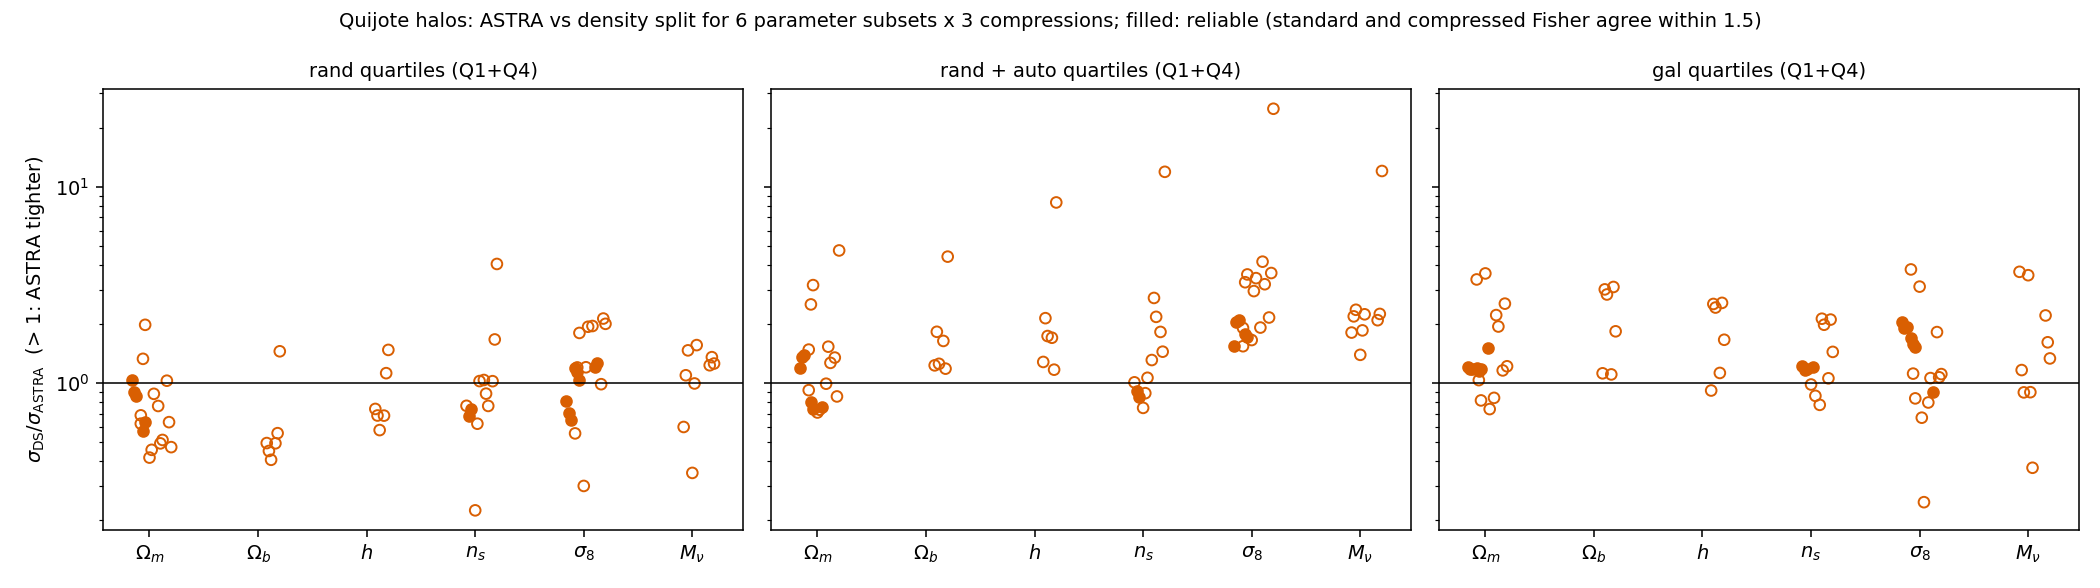
\includegraphics[width=\textwidth]{v2_quijote_subsets.png}
\caption{Halos de Quijote : $\sigma_{\rm DS}/\sigma_{\rm ASTRA}$ (au-dessus de 1 : ASTRA plus contraignant) pour six sous-ensembles de paramètres et trois compressions, pour les corrélations croisées des quartiles aléatoires (gauche), avec leurs auto-corrélations (centre), et les quartiles de halos (droite). Plein : prévisions fiables (estimateurs de Fisher standard et comprimé à moins d'un facteur 1.5) ; vide : dominées par le bruit des dérivées.}
\label{fig:qsubsets}
\end{figure*}

\subsection{Classes de toile cosmique ASTRA (Quijote)}
\label{sec:classes}

Pour tester si les classes ASTRA originales portent plus d'information que les quartiles, nous les avons mesurées sur Quijote, où les dérivées sont propres : 4000 réalisations fiducielles pour la covariance et les 500 paires de $\Omega_m$, $n_s$ et $\sigma_8$, avec les mêmes halos, points aléatoires et estimateurs que l'analyse en quartiles, et nous les avons comparées aux quartiles d'ASTRA et du density split mesurés sur les mêmes réalisations (bins de $10\Mpch$, $\ell=0,2$, $s\ge20\Mpch$). Comme les classes de vides et de nœuds sont presque vides pour les points aléatoires, les vecteurs de données de classes utilisent les feuillets et les filaments (ajouter les vides ne change rien).

\paragraph{Fractions de classes.} Les fractions de points dans chaque classe sont elles-mêmes sensibles à la cosmologie (Figure~\ref{fig:classes_resp}) : une variation de $\Omega_m$, $n_s$ ou $\sigma_8$ décale les fractions de feuillets et de filaments des points aléatoires de 0.3--1 fois leur dispersion entre réalisations, en sens opposés. Contrairement aux quartiles, dont les fractions sont fixées par construction, des seuils fixes laissent le volume de chaque environnement répondre à la cosmologie.

\paragraph{Information.} Le Tableau~\ref{tab:classes} et la Figure~\ref{fig:classes_fisher} comparent les classes aux quartiles d'ASTRA et du density split pour les trois compressions du vecteur de données utilisées dans la Section~\ref{sec:quijote}. Pour $(\Omega_m,\sigma_8)$, toutes les prévisions sont fiables. Avec les seules corrélations croisées, les classes portent à peu près autant d'information que les quartiles ASTRA, et moins que le density split sur $\sigma_8$. Avec les auto-corrélations, les classes sont la statistique la plus contraignante pour toutes les compressions : $\sigma(\sigma_8)$ est 2.1--3.0 fois plus petit qu'avec le density split et 1.35--1.45 fois plus petit qu'avec les quartiles ASTRA, et $\sigma(\Omega_m)$ 1.3--1.5 et $\sim1.1$ fois plus petit. Pour $(\Omega_m,n_s,\sigma_8)$, les classes avec auto-corrélations sont fiables pour toutes les compressions (et sont le seul vecteur de points aléatoires ASTRA fiable avec le binning le plus fin) ; leur avantage sur le density split reste d'un facteur 2.8--2.9 sur $\sigma_8$, mais diminue avec la compression sur $\Omega_m$ (1.0--1.5) et $n_s$ (1.2--1.85). Les classes des halos donnent un $\sigma(\Omega_m)$ inférieur de 15\% à celui des quartiles de halos mais un $\sigma(\sigma_8)$ plus grand.

\begin{table}[!htbp]
\centering\small
\begin{tabular}{lccc}
\toprule
compression & $\Omega_m$ & $n_s$ & $\sigma_8$ \\
\midrule
\multicolumn{4}{l}{$(\Omega_m,\sigma_8)$} \\
$10\Mpch$, $\ell=0,2$ & 1.28 & -- & 2.08 \\
$20\Mpch$, $\ell=0,2$ & 1.49 & -- & 2.95 \\
$20\Mpch$, $\ell=0$ & 1.52 & -- & 2.96 \\
\multicolumn{4}{l}{$(\Omega_m,n_s,\sigma_8)$} \\
$10\Mpch$, $\ell=0,2$ & 1.51$^*$ & 1.85$^*$ & 2.88$^*$ \\
$20\Mpch$, $\ell=0,2$ & 1.07 & 1.31 & 2.86 \\
$20\Mpch$, $\ell=0$ & 0.99 & 1.20 & 2.78 \\
\bottomrule
\end{tabular}
\caption{Quijote, 4000 réalisations fiducielles : $\sigma_{\rm DS}/\sigma_{\rm classes}$ pour les corrélations croisées et auto-corrélations des points aléatoires des quartiles du density split et des classes ASTRA (feuillets et filaments) ; au-dessus de 1 : classes plus contraignantes. $^*$ : density split de fiabilité marginale (rapport des estimateurs 1.5--1.6).}
\label{tab:classes}
\end{table}

\paragraph{Interprétation.} Le gain provient des auto-corrélations des deux classes et de la réponse de leurs volumes à la cosmologie, que des quartiles de taille égale suppriment par construction. L'avantage sur $\sigma_8$, un facteur 2--3 sur le density split, est robuste vis-à-vis de la compression, de l'ensemble de paramètres et du nombre de réalisations de la covariance ; l'avantage sur $\Omega_m$ et $n_s$ est plus faible et dépend de la compression. Pour une analyse de type DESI, cela exigerait un émulateur entraîné sur des statistiques de classes, c'est-à-dire de remesurer la suite d'émulation.

\begin{figure*}[!tp]
\centering
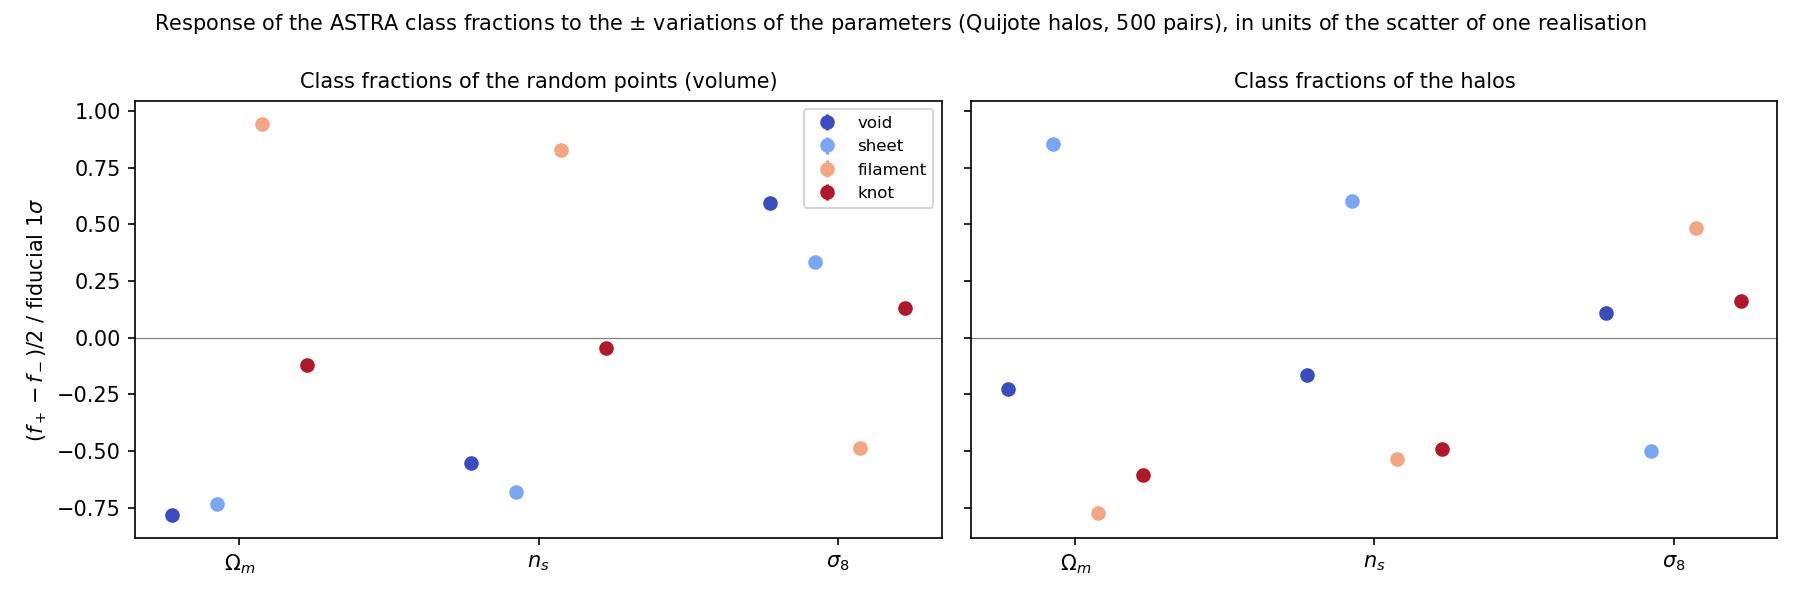
\includegraphics[width=\textwidth]{classes_response.png}
\caption{Réponse des fractions de classes ASTRA des points aléatoires (gauche) et des halos (droite) aux variations $\pm$ de $\Omega_m$, $n_s$ et $\sigma_8$ (Quijote, 500 paires), en unités de la dispersion d'une réalisation (barres d'erreur : erreur sur la moyenne, plus petite que les symboles).}
\label{fig:classes_resp}
\end{figure*}

\begin{figure*}[!tp]
\centering
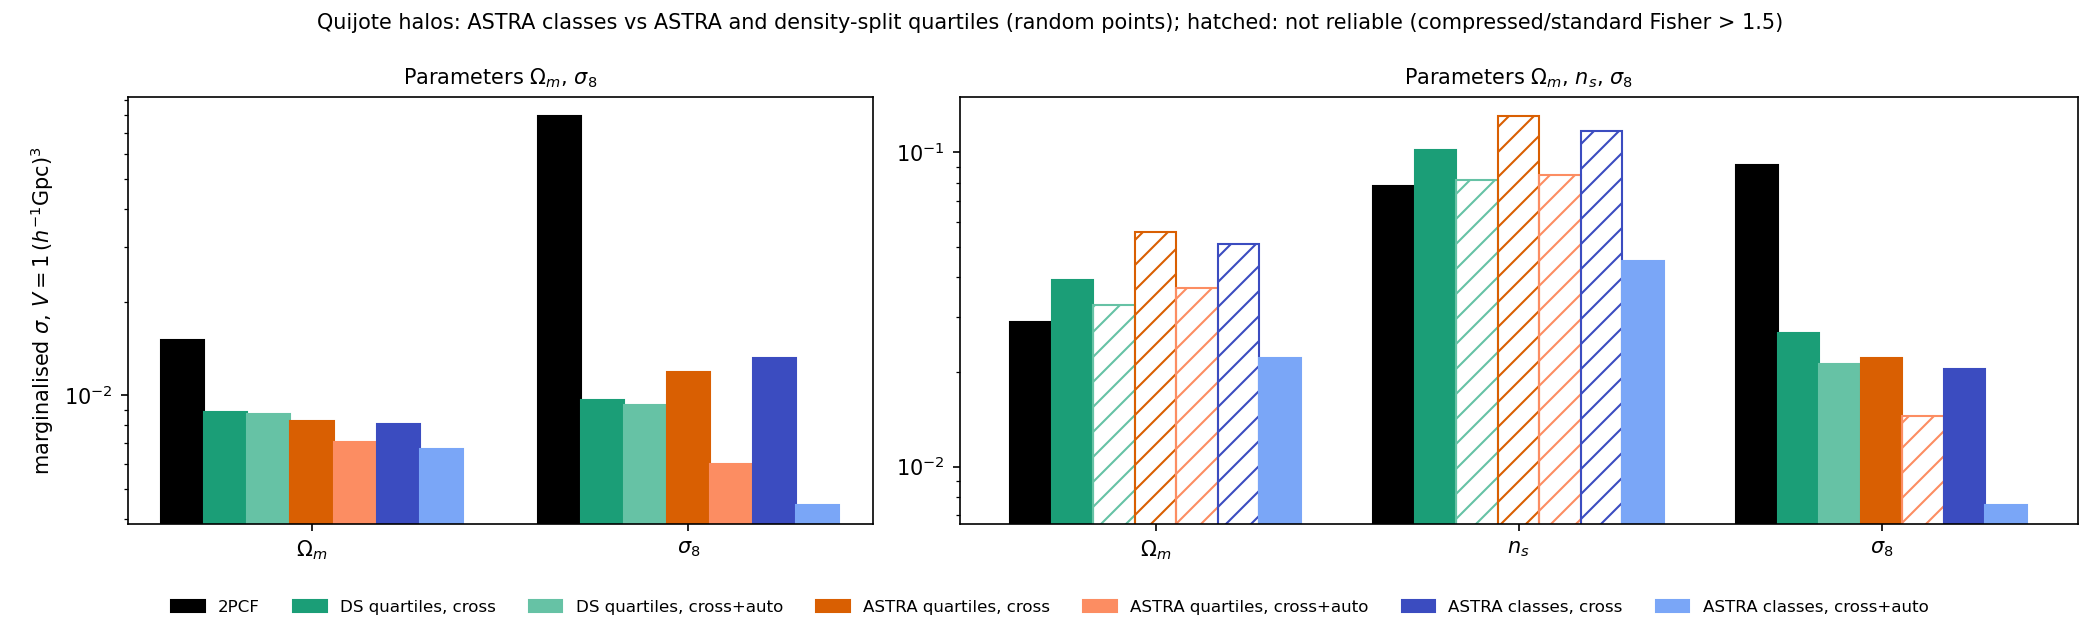
\includegraphics[width=\textwidth]{classes_fisher.png}
\caption{Halos de Quijote, $V=1\,(h^{-1}{\rm Gpc})^3$ : erreurs marginalisées pour $(\Omega_m,\sigma_8)$ (gauche) et $(\Omega_m,n_s,\sigma_8)$ (droite) de la 2PCF, des quartiles du density split et d'ASTRA des points aléatoires, et des classes ASTRA (feuillets et filaments), avec les seules corrélations croisées ou avec les auto-corrélations. Hachuré : non fiable (les estimateurs de Fisher comprimé et standard diffèrent de plus d'un facteur 1.5).}
\label{fig:classes_fisher}
\end{figure*}

\subsection{Inférence avec l'émulateur (MCMC)}
\label{sec:mcmc}

Les prévisions de Fisher supposent des posteriors gaussiens et sont locales. Pour tester la chaîne complète telle qu'elle serait appliquée aux données, nous avons échantillonné le posterior des 20 paramètres (8 cosmologiques, 12 de HOD) avec l'émulateur comme modèle : vraisemblance gaussienne avec la covariance officielle remise à l'échelle du volume des données plus l'erreur de l'émulateur, priors uniformes sur l'étendue d'entraînement, \texttt{emcee} avec 64 marcheurs et 8000 pas (Annexe~\ref{app:maths}). Les données sont des mesures que l'émulateur n'a jamais vues : un sous-volume de chacun de 2 catalogues des 8 cosmologies de test, et 8 sous-volumes de la boîte de base officielle de la cosmologie fiducielle, chacun analysé avec la 2PCF, l'ASTRA split, le density split et leurs combinaisons (120 chaînes).

Les posteriors sont non biaisés et calibrés ou légèrement conservateurs : la vérité se trouve à moins de $1\sigma$ de la moyenne du posterior dans 70--100\% des cas selon le paramètre (68\% attendus). Ils sont cependant à peine plus étroits que les priors (Figures~\ref{fig:mcmc} et~\ref{fig:mcmc_off}) : un volume de $(500\Mpch)^3$ avec 12 paramètres de HOD libres ne contraint que $\omega_{\rm cdm}$ et $\sigma_8$ au-delà du prior, de 10--15\%, et les statistiques diffèrent de quelques pour cent. Une première série d'exécutions sur la boîte complète de $(2\,h^{-1}{\rm Gpc})^3$ était limitée dans l'autre sens : l'erreur de l'émulateur (0.4--0.9 fois l'erreur statistique de ce volume) était aussi grande que l'erreur statistique, et masquait les différences entre statistiques. Distinguer les statistiques par l'inférence exige donc à la fois un grand volume et une erreur d'émulateur bien inférieure à l'erreur statistique de ce volume ; avec l'ensemble d'entraînement actuel ce n'est pas le cas (et la courbe d'apprentissage montre que davantage de catalogues du même type n'y changeraient rien), de sorte que la comparaison des méthodes repose sur les prévisions de Fisher. La chaîne d'inférence est validée et prête pour un ensemble d'entraînement plus grand ou moins bruité.

\begin{figure}[!htbp]
\centering
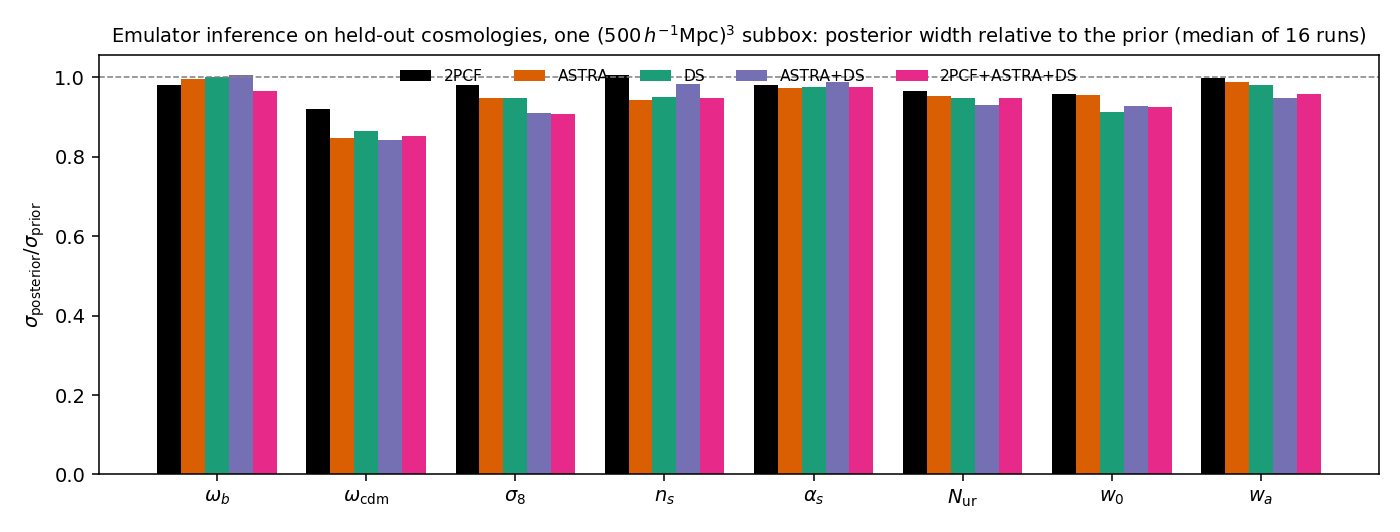
\includegraphics[width=\linewidth]{v2_mcmc_widths.png}
\caption{Inférence par l'émulateur sur des cosmologies exclues (un volume de $(500\Mpch)^3$, covariance officielle) : largeur du posterior relative à la largeur du prior, médiane de 16 exécutions, pour la 2PCF, l'ASTRA split, le density split et leurs combinaisons.}
\label{fig:mcmc}
\end{figure}

\begin{figure*}[!tp]
\centering
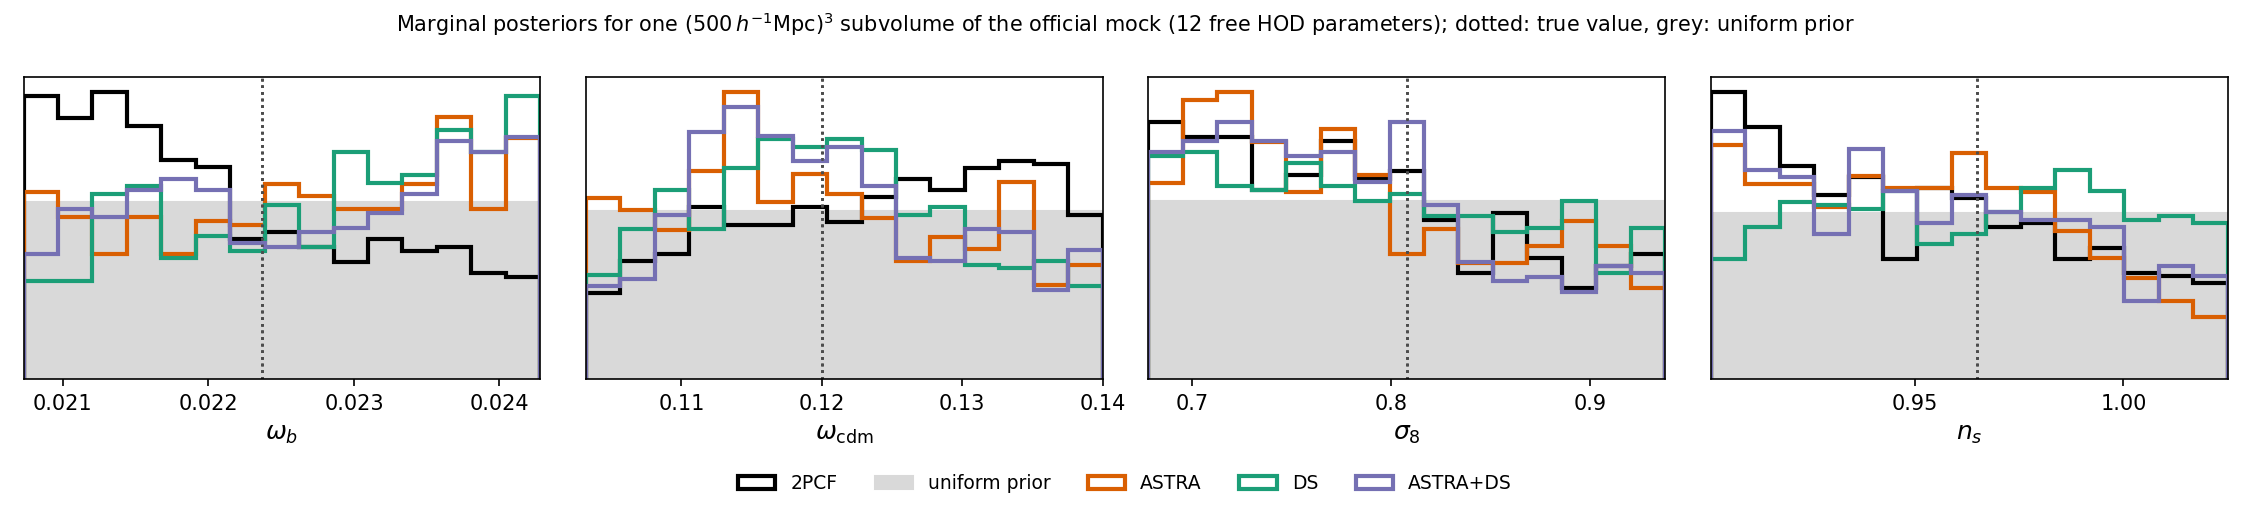
\includegraphics[width=\textwidth]{readable_mcmc_official.png}
\caption{Posteriors marginaux de quatre paramètres cosmologiques pour un sous-volume de $(500\Mpch)^3$ du mock officiel (cosmologie fiducielle, lignes pointillées), avec 12 paramètres de HOD libres, pour la 2PCF, l'ASTRA split, le density split et ASTRA + DS. À ce volume, tous les posteriors restent proches du prior uniforme (gris).}
\label{fig:mcmc_off}
\end{figure*}

